\documentclass[10pt,a4paper]{article}
\usepackage[margin=18mm]{geometry}
\usepackage{amsmath,amssymb,booktabs,array,graphicx,xcolor,hyperref,fancyhdr}
\usepackage[T1]{fontenc}
\usepackage{lmodern}
\hypersetup{colorlinks=true,urlcolor=blue,linkcolor=blue,pdftitle={The Price of Assuming You Will Know},pdfauthor={Hugo Lemonnier}}
\setlength{\parindent}{0pt}
\setlength{\parskip}{5pt}
\setlength{\tabcolsep}{3.3pt}
\setlength{\headheight}{14pt}
\emergencystretch=1.5em
\pagestyle{fancy}\fancyhf{}
\fancyhead[L]{\small Bayes-adaptive market making}
\fancyhead[R]{\small Separate research extension}
\fancyfoot[L]{\small Hugo Lemonnier}
\fancyfoot[R]{\small\thepage}
\newcommand{\E}{\mathbb E}
\newcommand{\BA}{\mathrm{BA}}
\newcommand{\PrimaryMean}{+0.004498}
\newcommand{\PrimaryLow}{-0.001066}
\newcommand{\PrimaryHigh}{+0.010062}
\newcommand{\PrimaryConclusion}{The prespecified economically meaningful improvement criterion is not met.}
\newcommand{\EvaluationMinutes}{10.8}
\newcommand{\GridWeights}{33}
\newcommand{\GridBeliefs}{65}
\newcommand{\GHNodes}{25}
\newcommand{\MaxHierarchyViolation}{3.1696e-05}

\begin{document}
\thispagestyle{empty}
{\LARGE\bfseries The Price of Assuming You Will Know}\par
\vspace{4pt}
{\large Bayes-adaptive market making under genuine model uncertainty}\par
Hugo Lemonnier \hfill 27 September 2026\par
\textit{Joint model-and-regime planning under persistent uncertainty.}

\section*{1. Question and result}
The original practical trader averages separately optimized, known-model action
values. It learns from public data during execution, but its planning score assumes
that the model will become known after the current decision. How costly is that
shortcut when regime persistence is uncertain? This extension implements a joint
model-and-regime Bellman recursion, derives model-revelation relaxations and
compares executable policies on fresh, paired market trajectories.

\textbf{Prespecified cold-start result.} Joint-belief minus weighted-Q net objective
is \textbf{\PrimaryMean}, with an empirical paired 95\% interval
\textbf{[\PrimaryLow,\ \PrimaryHigh]} per 30-decision episode.
\PrimaryConclusion{} The threshold is 0.002, the fee on one market execution
excluding its spread. Sampling uncertainty and numerical approximation error are
different: this interval describes the implemented policies, not a certified
optimality gap.

The experiment does not establish the registered economically meaningful improvement. The observed estimate and interval are retained even if other comparisons look more favorable.


\textbf{Fixed setting.} The model has $\theta=.35$ and unknown
$\kappa\in\{.002,.10\}$ with an equal prior, $T=30$ and inventory cap two.
Everything else---returns, selected-fill observation law, fees, spread, inventory
penalty, safe actions and terminal liquidation---is unchanged. The latent state
has four possibilities $(M,H)$, while the public signal has three values.
This is a restricted synthetic experiment, separate from the original campaign.

\begin{center}
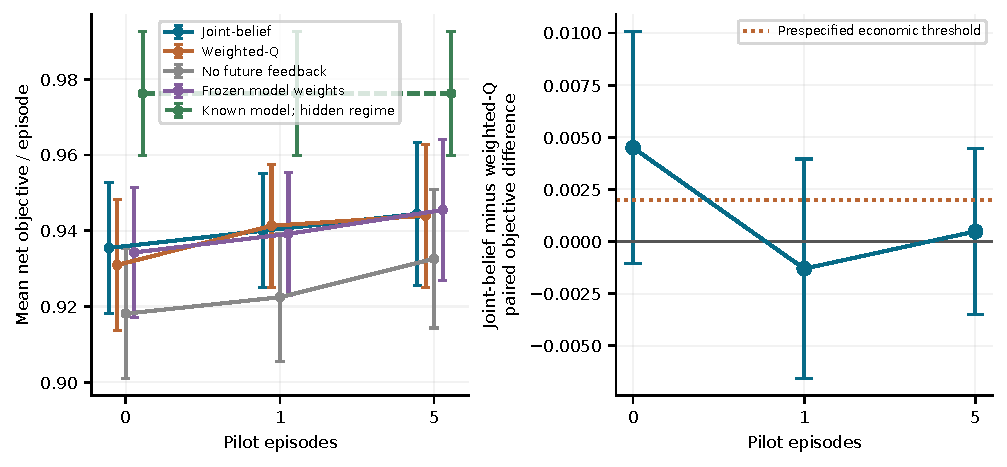
\includegraphics[width=\linewidth]{generated/economic_performance.pdf}
\end{center}
{\small\textbf{Figure 1.} Actual policy performance versus pilot information.
Left: policy means with ordinary empirical 95\% intervals; the known-model curve
is privileged about $M$ only, with $H$ still hidden. Right: paired joint-belief
minus weighted-Q differences, using the same trajectories and pilot at each
budget. Only the zero-pilot comparison is the primary hypothesis. The two other
budgets are prespecified sensitivity conditions. Numerical relaxation values are
reported separately on the next page.}

\textbf{What is preserved.} The original eight-page main report, eleven-page
appendix and canonical outcomes are retained.
This extension neither enlarges their deployment population nor revises their
reported results. Its conclusions concern only the experiment defined here.

{\small Implementation and computational checks used Codex with Astra and Sol agents.\par}

\newpage
\section*{2. Joint learning and the model-revelation shortcut}
Write $p_{j,h}=\Pr(M=j,H_t=h\mid\mathcal F_t)$, where $M$ is fixed during
an episode and $H_t\in\{-1,+1\}$ switches with probability $\kappa_j$.
The three coordinates are $w_j=\sum_h p_{j,h}$ and
$b_j=\Pr(H_t=+1\mid M=j,\mathcal F_t)$, with $w_2=1-w_1$.
The public state is $(q,x)$; $\mathcal A(q)$ requires every possible fill subset
to respect the inventory cap. Only submitted quotes produce fill observations.
For observed standardized return $z=(R-.03x)/.30$ and selected outcomes $f$,
the common-$\theta$ likelihood is
\begin{equation}
 \ell_h(z,f\mid x,a)=\prod_{(s,k)\in a}
 \Phi\!\left(\frac{(2f_s-1)[\tau_{s,k}(x)-h\theta sz]}
 {\sqrt{1-\theta^2}}\right),\qquad
 \tau_{s,k}(x)=\Phi^{-1}\!\bigl(p_{s,k}(x)\bigr).
\end{equation}
The empty product is one. Update from $H_t$'s observation \emph{before}
predicting $H_{t+1}$:
\begin{equation}
 \begin{gathered}
 m_j=(1-b_j)\ell_-+b_j\ell_+,\quad m=\sum_jw_jm_j,\quad
 w'_j=\frac{w_jm_j}{m},\\[-2pt]
 \widetilde b_j=\frac{b_j\ell_+}{m_j},\qquad
 b'_j=\kappa_j+(1-2\kappa_j)\widetilde b_j,
 \qquad p'_{j,+}=w'_jb'_j .
 \end{gathered}
\end{equation}
Zero-mass branches have no contribution. Let $r(q,x,p,a)$ denote exact expected
marked-to-midpoint wealth change minus the pre-decision $.002q^2$ penalty,
including execution fees. For $n$ remaining decisions, terminal liquidation
gives $V_0(q,x,p)=-.027|q|$. With $q'=q'(q,a,f)$, the exact recursion is
\begin{equation}
 V_n=\max_{a\in\mathcal A(q)}\left\{
 r(q,x,p,a)+\sum_f\int_{\mathbb R}\phi(z)m(z,f)
       \sum_{x'}K_{xx'}V_{n-1}(q',x',p')\,dz\right\}
 \equiv (\mathcal B V_{n-1})(q,x,p).
\end{equation}
The Gaussian density cancels from posterior ratios but remains in this
expectation. At cold start $b_1=b_2=1/2$, $m_1=m_2$ for every action and
observation: the first observation has exactly zero model information.

Let $V_{j,n}$ and $Q_{j,n}$ be exact controls knowing $M=j$ while still filtering
$H$. Define $U_n^d$ by revealing $M$ just before decision $d+1$; for $d\ge n$,
there is no useful revelation. Then
\begin{equation}
 \begin{gathered}
 U_n^0(q,x,p)=\sum_j w_jV_{j,n}(q,x,b_j),\qquad
 U_n^d=\mathcal B U_{n-1}^{d-1}\quad(d\ge1),\\[-2pt]
 U_n^1(q,x,p)=\max_{a\in\mathcal A(q)}\sum_jw_jQ_{j,n}(q,x,b_j).
 \end{gathered}
\end{equation}
Indeed, conditioning on the common first action and observation gives
$m w'_j=w_jm_j$; substituting this into its continuation yields the weighted
known-model Q score. Earlier revelation can emulate later revelation by ignoring
the extra label. It follows that
\begin{equation}
 U_n^0\ge U_n^1\ge U_n^2\ge\cdots\ge U_n^n=V_n.
\end{equation}
These inequalities concern exact planning values. A trader repeatedly maximizing
weighted Q receives no actual revelation; its executed value need not equal
$U_n^1$. Interpolation and quadrature produce approximations to these quantities,
not certified numerical bounds. The full proofs and conservative error
allowances are in \texttt{THEORY.md}.


\begin{center}\small
\begin{tabular}{lrrr}\toprule
Approximate planning quantity & Pilot 0 & Pilot 1 & Pilot 5\\\midrule
$U^0$: model known at entry & 0.980878 & 0.973269 & 0.963642\\
$U^1$: revealed after 1 decision & 0.980878 & 0.973269 & 0.963642\\
$U^2$: after 2 decisions & 0.980616 & 0.973045 & 0.963489\\
$U^3$: after 3 decisions & 0.980370 & 0.972820 & 0.963332\\
$V^{\rm BA}$: no revelation & 0.938274 & 0.934593 & 0.935156\\
\bottomrule\end{tabular}

\end{center}
{\small\textbf{Table 1.} Numerical planning values at $q=x=0$, fresh conditional
regime priors $b_1=b_2=.5$, and the model posterior fitted from each pilot.
Entries average over the balanced pilot population. These are approximate
relaxed or Bellman objectives, \emph{not} policy rollout returns and \emph{not}
certified numerical upper bounds. $U^1$ is evaluated directly from weighted
known-model Q values; the stored nodal relaxation has a distinct interpolation.
The largest observed local hierarchy reversal is \MaxHierarchyViolation{}.}

\textbf{Why the hierarchy is useful.} Each delay removes fictitious information
while retaining the physical market and admissible actions. The optimizing first
action may change. The exact hierarchy applies to prior-weighted values, not
individual outcomes or true-model strata. It explains optimism in weighted-Q
planning. Uncertified numerical relaxation values and Monte Carlo returns do not
certify near-optimality.

At cold start, the numerical $U^1$ minus achieved weighted-Q mean is +0.049920; delaying revelation to $U^3$ reduces the corresponding diagnostic to +0.049412. These differences combine planning approximation and Monte Carlo error. They are not certified upper bounds on the heuristic's suboptimality. The complete budget-by-policy diagnostics are exported in the accompanying tables.


\newpage
\section*{3. A fixed experiment that can contradict the hypothesis}
Each true model has 30 independent replicates. Every replicate supplies five
independent 30-step uniform-safe-action pilot episodes, and 1,000 fresh evaluation
episodes. The budgets use no pilot, the first pilot, and all five. The model is
fixed within a replicate; every episode starts with a new hidden regime.
Evaluation resets the conditional regime beliefs to one half, retains only the
pilot model posterior, and never transfers evaluation learning to another episode.

Five policies share each pilot and market tape: joint-belief planning, weighted-Q,
no future feedback, frozen future model weights, and the known-model reference.
Every feasible policy filters all permitted feedback online. The two suppressions
change hypothetical planning updates, not the observations supplied at runtime.
Only the privileged reference receives the true model label; it never sees $H$.

There are \textbf{60,000 paired market trajectories and 900,000 policy-episode
records}. Their reuse across policies and pilot budgets does not create additional
independent markets. Pairing uses the complete model/replicate/episode/budget key.
Within each model, paired episode differences are averaged by replicate; the two
stratum means receive equal weight. Welch intervals estimate between-replicate
uncertainty. Missing cells, broken pairs, duplicate keys, insufficient replicates
and nonfinite outcomes are rejected before inference.

\begin{center}\scriptsize
\begin{tabular}{llrr}\toprule
Pilot & Comparison & Objective difference & Net-PnL difference\\\midrule
0 & Joint -- weighted-Q & +0.00450 [-0.00447, +0.01346] & +0.00771 [-0.00123, +0.01665]\\
0 & Joint -- no feedback & +0.01735 [+0.00660, +0.02809] & +0.00969 [-0.00104, +0.02041]\\
0 & Joint -- frozen weights & +0.00118 [-0.00558, +0.00795] & +0.00096 [-0.00581, +0.00773]\\
0 & Known model -- joint & +0.04079 [+0.02836, +0.05323] & +0.03876 [+0.02635, +0.05116]\\
1 & Joint -- weighted-Q & -0.00131 [-0.00979, +0.00718] & +0.00136 [-0.00716, +0.00988]\\
1 & Joint -- no feedback & +0.01756 [+0.00666, +0.02846] & +0.01001 [-0.00098, +0.02100]\\
1 & Joint -- frozen weights & +0.00083 [-0.00650, +0.00816] & +0.00054 [-0.00678, +0.00785]\\
1 & Known model -- joint & +0.03624 [+0.02244, +0.05004] & +0.03480 [+0.02098, +0.04862]\\
5 & Joint -- weighted-Q & +0.00048 [-0.00596, +0.00693] & +0.00219 [-0.00428, +0.00866]\\
5 & Joint -- no feedback & +0.01186 [-0.00075, +0.02448] & +0.00495 [-0.00773, +0.01763]\\
5 & Joint -- frozen weights & -0.00102 [-0.00577, +0.00372] & -0.00125 [-0.00601, +0.00350]\\
5 & Known model -- joint & +0.03178 [+0.01420, +0.04936] & +0.03124 [+0.01361, +0.04887]\\
\bottomrule\end{tabular}

\end{center}
{\small\textbf{Table 2.} All 24 prespecified supplementary contrasts: four
comparisons, three pilot budgets and two metrics. Brackets are Bonferroni-adjusted
empirical intervals for this family. The ordinary primary interval is stated on
page 1; it is not replaced by a favorable supplementary result. Net PnL includes
execution and liquidation costs; net objective additionally deducts the original
pre-decision inventory penalty.}

\begin{center}
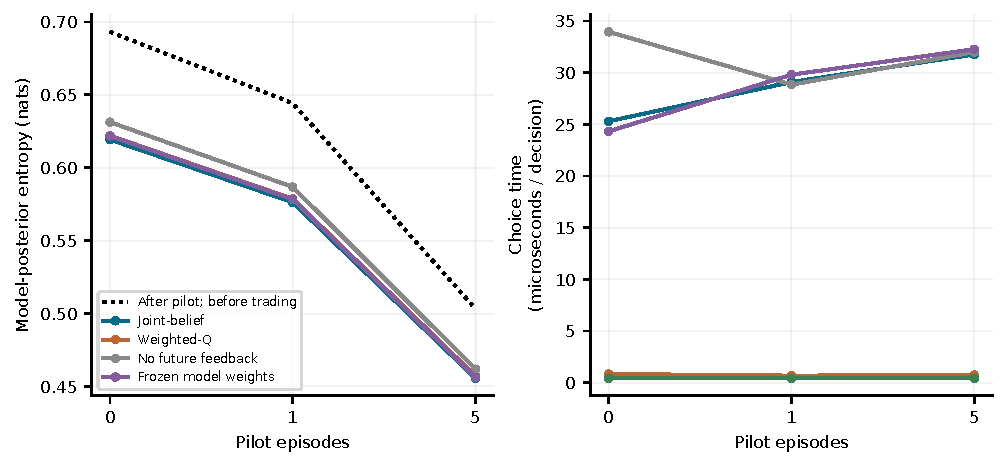
\includegraphics[width=\linewidth]{generated/information_and_compute.pdf}
\end{center}
{\small\textbf{Figure 2.} Left: model-posterior entropy after the pilot and after
trading; lower entropy alone is not evidence of economic benefit. Right: measured
policy-choice time, including table access on this numerical build. These timings
are workload observations on a shared machine, not universal latency guarantees.
The known-model reference's shadow public posterior is excluded from the entropy
plot because its own model uncertainty is zero.}

\newpage
\section*{4. What a controlled decision can establish}
With common $\theta$, an observation depends on the model only through the current
hidden regime. Thus $M\to H_t\to O_t$ conditional on public history and action,
and
\[
 I(M,H_t;O_t)=I(H_t;O_t)=I(M;O_t)+I(H_t;O_t\mid M).
\]
At cold start, $b_1=b_2=.5$: every action's first observation has identical
likelihood under both models, so its model information is exactly zero. Regime
updating followed by different persistence transitions separates the conditional
beliefs; later observations can then identify the model. Parameter information
comes from temporal dependence, not a direct model label in a fill.

The explanation search was fixed before evaluation: 60,000 public states reached
by uniform-safe actions, plus 77,430 fixed arbitrary belief/horizon probes.
It screens action disagreements, ranks by declared score margins and examines a
bounded ordered candidate set, without choosing favorable realized PnL paths.
Reached and arbitrary-prior states are identified separately.

The fixed search screened 137,430 states and directly checked 512 distinct disagreements. It found 223 cases meeting the complete action-margin and cross-refinement witness criterion.
A refinement-stable witness is candidate 48408, with $n=12$, $q=2$, $x=1$ and $p=(0.025081, 0.461728, 0.315619, 0.197572)$. It is reached by the separate public exploration process, not selected from policy evaluation.
The direct joint-belief backup selects ask deep (ID 2); weighted-Q selects abstain (ID 0); keeping the same joint-belief continuation but freezing model weights selects abstain (ID 0).
\begin{center}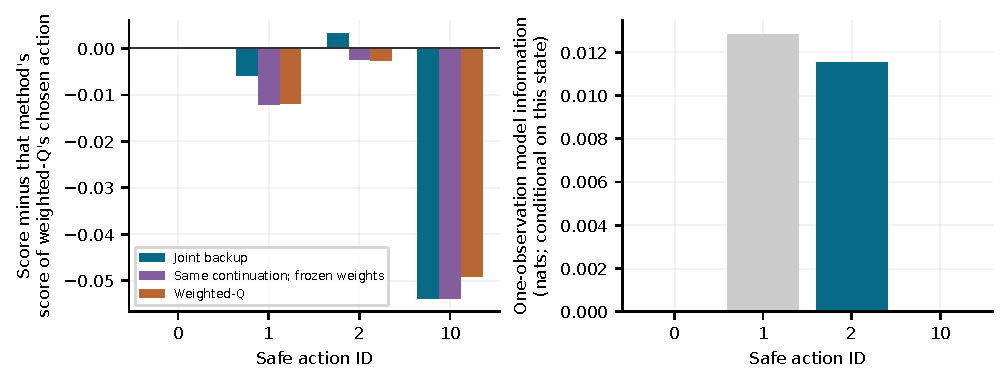
\includegraphics[width=\linewidth]{generated/action_explanation.pdf}\end{center}
{\small\textbf{Decision diagnostic.} Each score is centered on that same method's score of the weighted-Q action; absolute relaxed and feasible values are not subtracted. Positive information does not itself establish economic benefit.}
\begin{center}\small\begin{tabular}{lrr}\toprule
Quantity & Joint-belief choice & Weighted-Q choice\\\midrule
Immediate expected reward & +0.0460881 & +0.0520000\\
Model information (nats) & +0.0115330 & +0.0000000\\
Regime information conditional on model & +0.0214307 & +0.0000000\\
\bottomrule\end{tabular}\end{center}


\textbf{Attribution limit.} The matched diagnostic keeps immediate rewards,
outcome probabilities, inventory transitions, conditional regime updates and the
same joint-belief continuation fixed. It freezes only the model weights at the
next hypothetical planning boundary. This is an artificial computational
intervention, not a Bayesian observation deletion or an information bound.
When $b_1\ne b_2$, preserving the likelihood ratio needed by both regime filters
also preserves the model Bayes factor:
\[
\frac{m_1}{m_2}=\frac{1-b_1+b_1R}{1-b_2+b_2R},\qquad R=\ell_+/\ell_-.
\]
Freezing model weights changes the aggregate regime forecast as well. A stable
decision reversal establishes sensitivity to that update; it does not isolate
a pure model-information channel. Economic value requires the paired policy
comparison, not just entropy reduction or a selected negative immediate reward.

\newpage
\section*{5. Numerical accuracy and reproducibility}
The solver uses float64 product coordinates $(w,b_1,b_2)$, trilinear interpolation
in physical probabilities, analytic expected one-step rewards and positive
Gauss--Hermite quadrature. Model-weight nodes are uniform; conditional-regime
nodes follow $b(u)=\sin^2(\pi u/2)$, concentrating resolution near the endpoints.
This numerical-only amendment follows retained uniform-mesh failures and was
frozen before local final evaluation, with unchanged probes and tolerances.
The selected joint grid is $\GridWeights\times\GridBeliefs\times\GridBeliefs$
with \GHNodes{} quadrature nodes. The independent known-model scalar references
use 321 beliefs and 161 nodes, compared with separate belief and quadrature
refinements. The absolute tie tolerance is $10^{-12}$; the lowest safe action ID
wins, and the Bellman value uses that selected action's Q.

\begin{center}
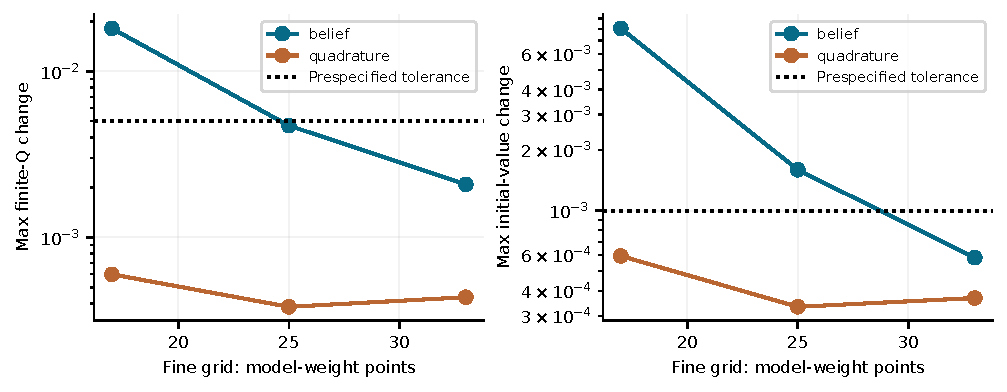
\includegraphics[width=\linewidth]{generated/numerical_refinement.pdf}
\end{center}
{\small\textbf{Figure 3.} Independent refinement axes, retaining failures.
All 30 remaining horizons use identical fixed off-grid probes. Acceptance requires
initial value change at most .001, probe value and finite-Q change at most .005,
and robust-action disagreement at most .005 when the finer gap exceeds .001.
The same rule covers six value modes and all three joint action-score modes.}

The final two independently varied axes both satisfy the frozen rule. Earlier failed meshes and the resource-driven V1 interruption remain in the evidence.

For the belief comparison, maximum initial-value, probe-value and finite-Q changes are 0.000583643, 0.00202047 and 0.00208867; the robust-action disagreement fraction is 0.

For the quadrature comparison, maximum initial-value, probe-value and finite-Q changes are 0.000368036, 0.000391736 and 0.000436629; the robust-action disagreement fraction is 0.

The selected-family conservative one-sided allowance at $T=30$ is 9.46506, and the two-sided off-grid allowance is 15.50378 objective units. They are much larger than .002; their floating evaluation is not an interval-arithmetic certificate.


\textbf{A proved envelope, not a small optimality certificate.}
For a fixed policy tree, its expected payoff is linear in the four-state prior.
The exact optimal value is therefore convex. The product-grid corner weights
have the correct joint-mass barycenter, giving an upper interpolation of exact
nodal values. Quadrature error has no known sign, so this fact does not make the
computed tables certified upper bounds.

A conservative conditional expected stage-reward bound is $r_*=.231$, with
terminal payoff in $[-.054,0]$. For $D_n=.231n+.027$, exact values satisfy
$|V_n(p)-V_n(\bar p)|\le D_n\|p-\bar p\|_1$. Grid and observation-integration
errors can consequently be bounded using the mesh widths and the Wasserstein
distance between the normal law and its quadrature measure. The full derivation,
computed allowances and omitted floating-arithmetic certification are explicit
in \href{Mathematical_Appendix.pdf}{the mathematical appendix} and
\texttt{THEORY.md}. These conservative bounds are too wide to certify the
economic threshold. Refinement and independent rollouts give useful numerical
evidence, while remaining logically distinct from a uniform mathematical error bound.

\newpage
\section*{6. Validation, interpretation and review entry point}
The independent verifier reconstructs all 900,000 outcome records, all 27 million policy decisions, 108,000 posterior-trace rows and 60 pilot sets from the saved primitive tapes and permitted public feedback. It imports neither the producer's runner nor its statistical routines. All 24 supplementary contrasts, 30 policy means and 180 initial planning-value rows reconcile. The largest absolute ledger discrepancy is 2.50111e-12; the largest public-trace discrepancy is 1.59162e-12.

A fresh process builds the selected family in a previously nonexistent cache. All eleven array-content records and actual file hashes match the reference build. A separate smoke process produces 720 policy records on 48 paired tapes; its pilots, tapes, actions, outcomes, traces, planning values and summaries match exactly, with all 21,600 decisions independently replayed. Measured timing metadata retains its new identity. These are repeated checks of the same seeds, not independent economic observations.

The final economic execution took 10.8 minutes on the recorded stack; the selected-resolution cold reproduction took 28.3 minutes. Both durations are workload observations. The actual review archive has its own packaging and extracted-execution receipt; those checks are separate from numerical and statistical validation.

The cold-reproduction duration sums active command execution and excludes the
pause for recovering the preserved original archive's local path. The failed
path check and its successful continuation remain in the evidence; no second
cold build is claimed.

\subsection*{Interpretation and limits}
This extension supplies a different decision recursion and a testable account of
the weighted-Q shortcut. It does not claim to invent Bayes-adaptive control:
model uncertainty and hidden-state uncertainty are treated jointly in the
Bayes-adaptive POMDP literature [1], and information relaxations and approximate
POMDP value methods have an established history [2,3]. Our contribution is the
specialized model-only revelation interpretation, its implementation in this
selected-feedback trading model, and the separately registered evidence.

The experiment does not establish the registered economically meaningful improvement. The observed estimate and interval are retained even if other comparisons look more favorable. The numerical relaxation ladder explains the shortcut's information optimism, but the present conservative error envelope does not prove a small global optimality gap. The fixed action search supplies 223 qualifying cases; their frequency in a designed search is not an estimate of their prevalence under either policy.


The scope is two correctly specified persistence models with known dependence
magnitude, a finite horizon and small inventory. It establishes neither commercial
trading validity nor a result under off-grid parameters or arbitrary shifts.
Pilot uncertainty is genuine here, but the known finite support remains an
assumption. Entropy, relaxed planning optimism and realized policy benefit answer
different questions and cannot be substituted for one another.

\subsection*{Reproduction}
The public repository contains the protocol, source, numerical refinement,
pilots, evaluation tapes, actions, outcomes, posterior traces and statistical
tables. \texttt{REPRODUCING.md} gives installation and mathematical checks.
Four authenticated byte chunks restore the complete compressed ledger.

Recorded evidence belongs to its original numerical build. Fresh runs bind
their own source, tables and outputs. Regenerable control arrays are excluded;
their specifications and content fingerprints are retained. The small E2E
reproduction verifies installation and integration, not the numerical precision
of a new full campaign.

\subsection*{References and authorship}
\begin{enumerate}\small
\item S. Ross, B. Chaib-draa and J. Pineau (2007),
\href{https://papers.nips.cc/paper_files/paper/2007/file/3b3dbaf68507998acd6a5a5254ab2d76-Paper.pdf}{Bayes-Adaptive POMDPs}, NeurIPS.
\item M. Hauskrecht (2000),
\href{https://jair.org/index.php/jair/article/download/10262/24449}{Value-Function Approximations for Partially Observable Markov Decision Processes}, JAIR 13, 33--94.
\item R. D. Smallwood and E. J. Sondik (1973),
\href{https://pubsonline.informs.org/doi/10.1287/opre.21.5.1071}{The Optimal Control of Partially Observable Markov Processes over a Finite Horizon}, Operations Research 21(5), 1071--1088.
\end{enumerate}
\end{document}
